\documentclass{article}
\pagestyle{empty}
\usepackage[margin=1in]{geometry}
\usepackage{hyperref}
\usepackage{graphicx}
\usepackage{multicol}
\setlength{\parindent}{0in}
\setlength{\parskip}{1em}
\begin{document}

\centerline{\large\bf CSCI 321, 3D Game Specs, Spring 2016}
\centerline{\bf Due date: Wednesday, May 18, Midnight}

\begin{itemize}
  \item
Reread the 2D game specifications for general things I'll look for in
your game.  However, since 3D is generally {\em much} harder than 2D,
much less is expected of your game.  Splash screens, scoreboards,
health bars, and most of the other non-diegetic material does not have
to be implemented.  One interesting level is plenty.  
\item
If you've used images, sounds, or other resources, make sure you pack
them into your blend file with the
\verb+File->External Data->Pack All into .blend+ menu item.  To make
sure you've done this you may want to try to open your game on a
different computer before submitting it.  Or just move or delete all
the folders with resources and reopen your game.
\item
Set up a new screen layout, called {\bf PlayGame}, by pressing the
$+$-key on the drop-down menu that has the builtin screen layouts
(Default, Animation, {\em etc.}), renaming it, and then setting it up
with just one large 3D window on the left, and a narrow text window on
the right, as in this figure:

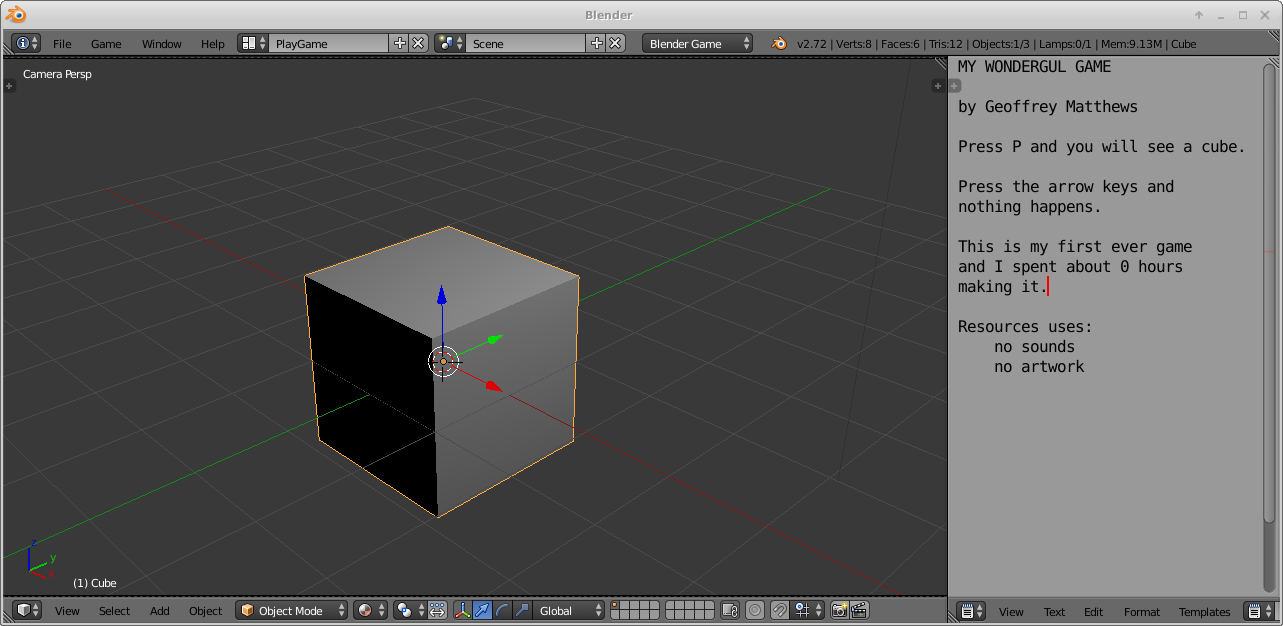
\includegraphics[width=\textwidth]{blendergameplaysetup.png}
  
Set up the 3D window so it is ready to play with a single press of the
P-key:  textured mode, camera view, {\em etc.}
You can provide the name, in-game help, {\em etc.} in the text window,
so that the manual does not have to be consulted.  

\item {\bf Save the game in this configuration!}  So that when I open
  it this will be the first thing I see.

\item Also produce a user's manual, as before, nicely formatted.  Please let
me know here all the special features and glorious whatnots you put in
your game; tell me what you spent your time on, so I won't miss it
when I'm deciding your grade.  A programmer's guide is not necessary
unless you wrote code (python scripts) for your game.
\end{itemize}


\end{document}
\end
